\section{Benchmarking of Planners}
\localtableofcontents
In the previous sections, we found out the path plans for optimal welding using the 2Dof rotary table. We also addressed the problem of reachability and showed how it can be overcome using the table. In this chapter we will delve into the effects of  table optimization on the motion planners, in terms of time taken to generate a plan, correctness of solution generated and best cost(lowest) of solution found. We consider 2 different scenarios, for benchmarking the planners first without optimizing the table position and next with the table optimization turned on. The following criteria were considered for comparing the results of the two use cases. The criteria are defined in \citet{moll2015benchmarking-motion-planning-algorithms}:
\begin{itemize}
	\item Time of Planning: The amount of time spent in planning to connect start and goal point. A key point to be noted here is that for optimizing planners like RRT start, the planners continues to find solutions which are more optimized, until it runs out of time [\citet{moll2015benchmarking-motion-planning-algorithms}]. 
	\item Status of Plans Generated: This metric only shows if a planner has been able to successfully generate plans for every iteration that it ran.
	\item Best Cost of Plans Generated: This metric determines the cost of the planned path. Currently only RRT star can record the cost value of the planned paths [\citet{moll2015benchmarking-motion-planning-algorithms}].
\end{itemize}
The use cases are illustrated in figures (\ref{bm:uc1} and \ref{bm:uc2}).
The configuration details of the planners are presented in the appendix section.
\begin{figure}[!htbp] %  figure placement: here, top, bottom, or page
	\centering
	\begin{subfigure}[b]{0.4\textwidth}
		\frame{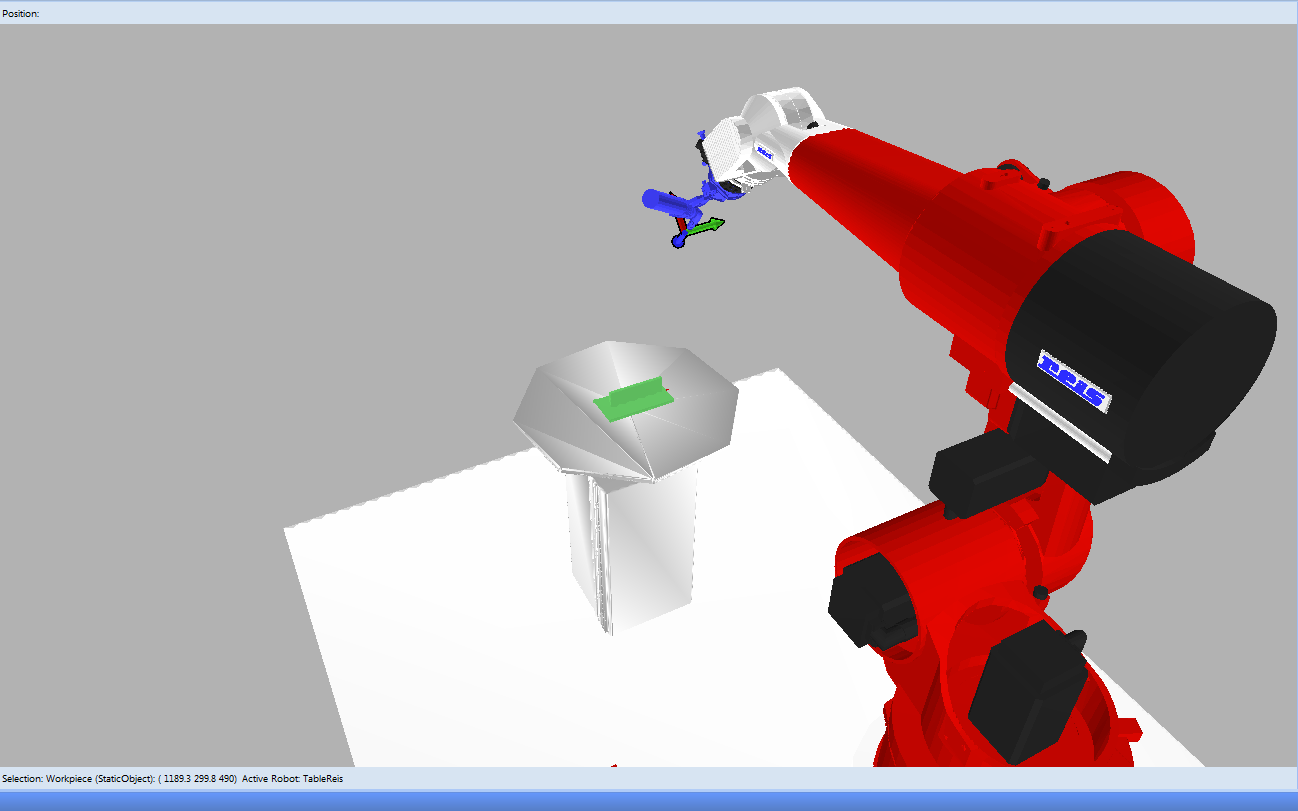
\includegraphics[width=1\textwidth,height=0.2\textheight]{images/un_opt_bnch.png}}
		\caption{Use Case Without Table Position Optimization}  
		\label{bm:uc1}
	\end{subfigure}
	\begin{subfigure}[b]{0.4\textwidth}
		\frame{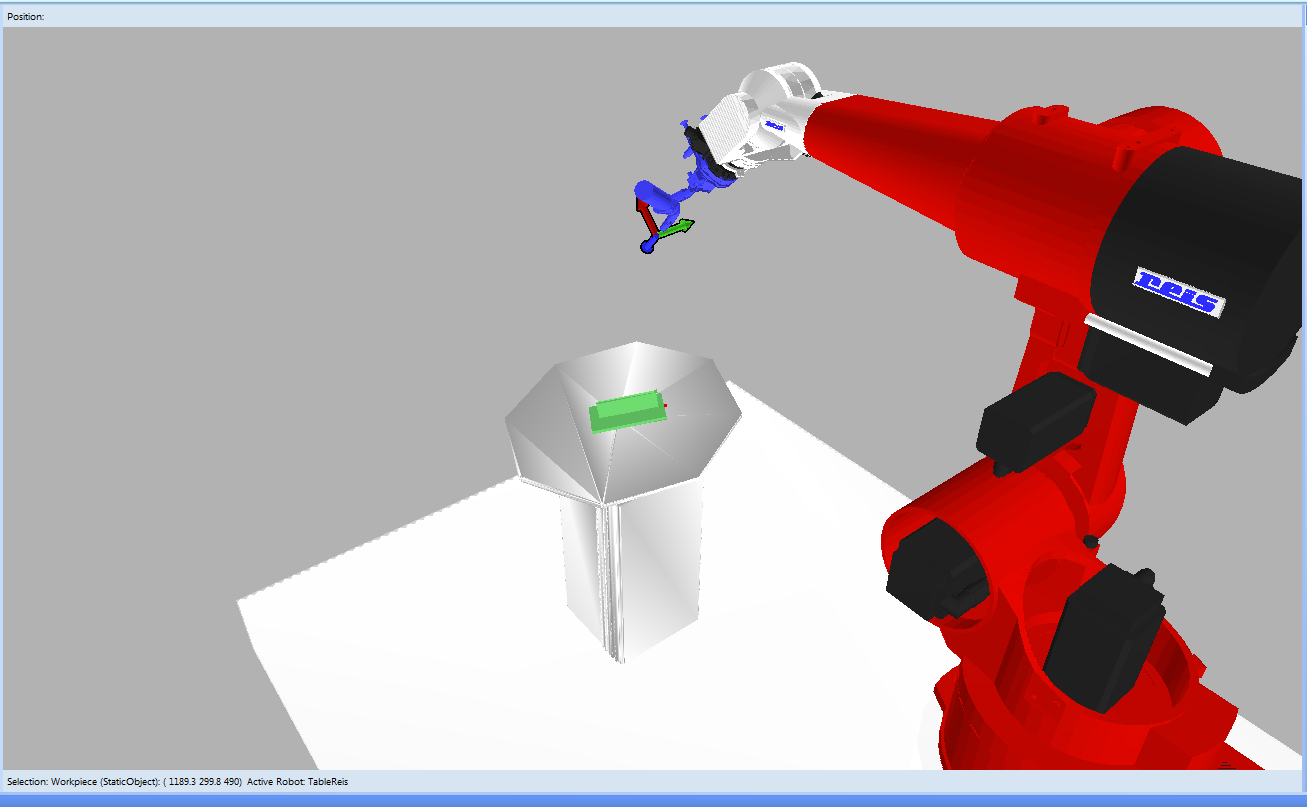
\includegraphics[width=1\textwidth,height=0.2\textheight]{images/opt_bnch.png}}
		\caption{Use Case With Table Position Optimization}  
		\label{bm:uc2}
	\end{subfigure}	
	\caption{Benchmarking Use Cases}
	\label{bm:uc}
\end{figure}
\clearpage 
The parameters for benchmarking are as follows:
\begin{itemize}
	\item No. of Iterations for each planner: 20
	\item Maximum allowable time limit for each iteration: 120sec
	\item Maximum allocated memory for each planner for each iteration: 200MB
	\item Planners used: RRT*, TRRT, KPIECE1, LBKPIECE1, SBL.
\end{itemize}
The time taken by the planners different planners, were in different ranges, hence we plot the times for RRTstar and TRRT separately and group the plots for SBL,KPIECE1,LBKPIECE1. 
\begin{figure}[!htbp] %  figure placement: here, top, bottom, or page
	\centering
	\frame{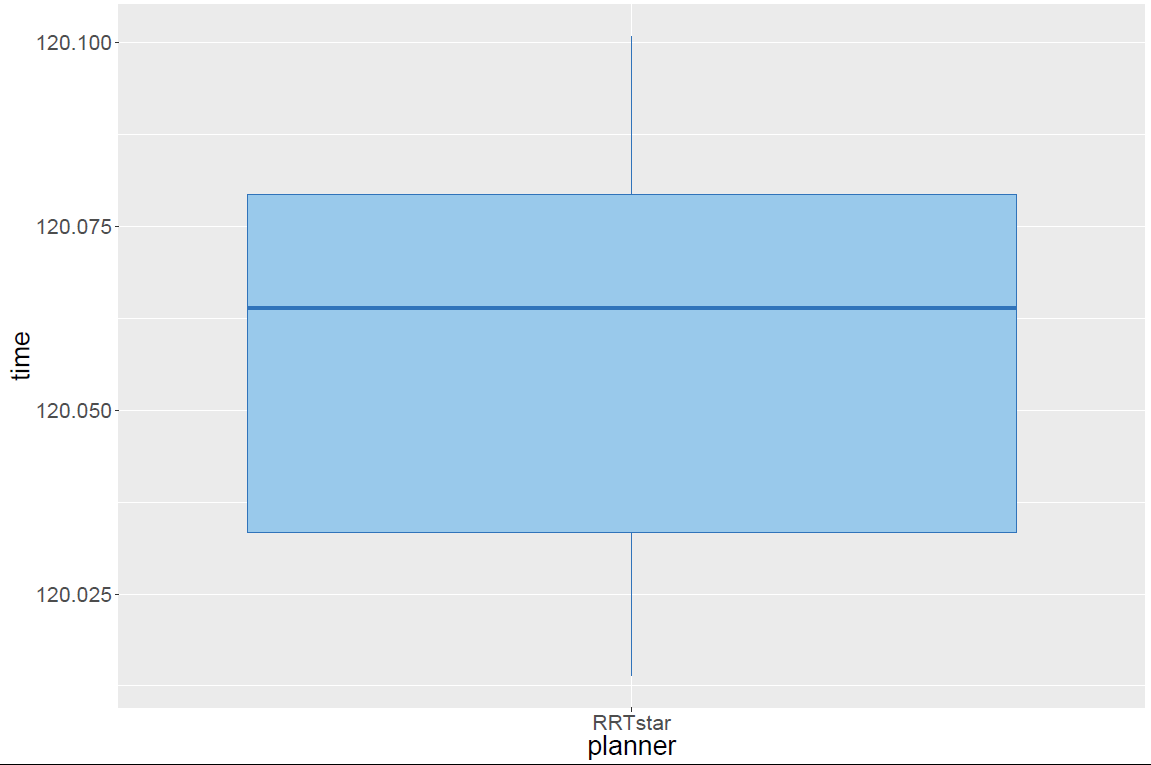
\includegraphics[width=0.8\textwidth,scale=0.6]{images/Timerrtuop.png}}
	\caption{Time of Planning RRT*: Unoptimized}
	\label{fig:tc1}
\end{figure}
\begin{figure}[!htbp] %  figure placement: here, top, bottom, or page
	\centering
	\frame{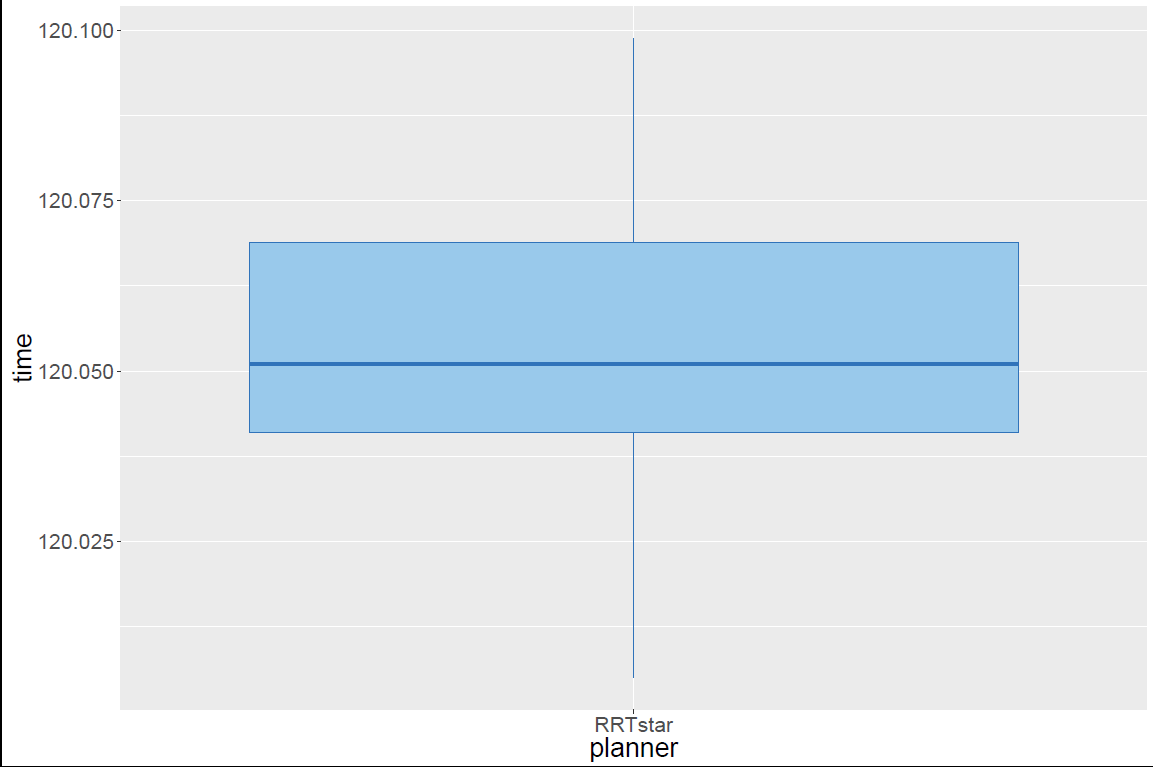
\includegraphics[width=0.8\textwidth,scale=0.6]{images/Timerrtop.png}}
	\caption{Time of Planning RRT*: Optimized}
	\label{fig:tc2}
\end{figure}
\begin{figure}[!htbp] %  figure placement: here, top, bottom, or page
	\centering
	\frame{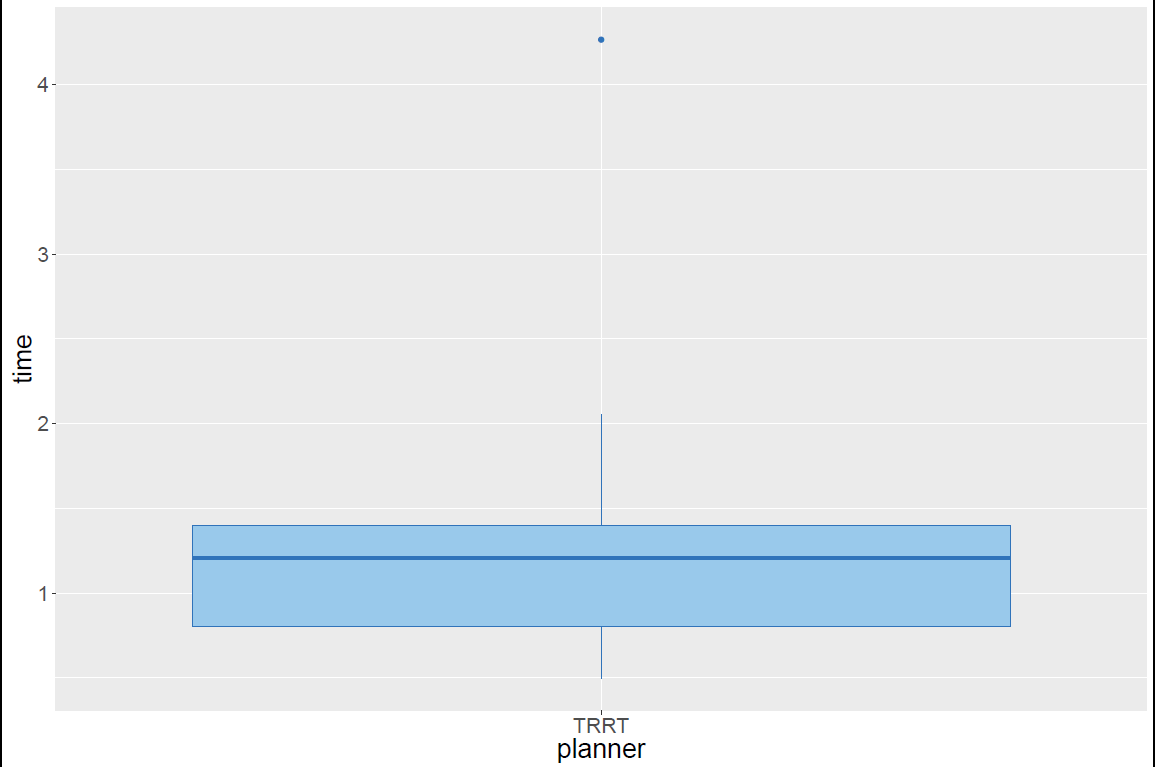
\includegraphics[width=0.8\textwidth,scale=0.6]{images/trrtuop.png}}
	\caption{Time of Planning TRRT: Unoptimized}
	\label{fig:tc3}
\end{figure}
\begin{figure}[!htbp] %  figure placement: here, top, bottom, or page
	\centering
	\frame{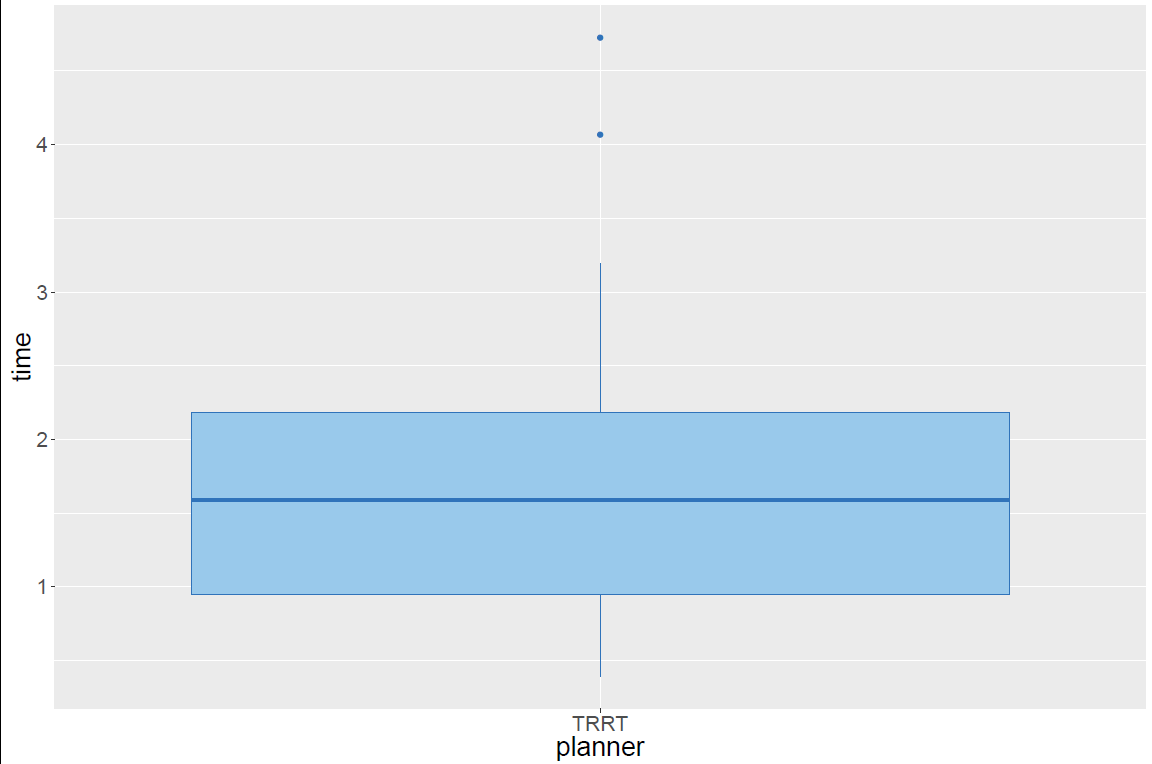
\includegraphics[width=0.8\textwidth,scale=0.6]{images/trrtop.png}}
	\caption{Time of Planning TRRT: Optimized}
	\label{fig:tc4}
\end{figure}
\begin{figure}[!htbp] %  figure placement: here, top, bottom, or page
	\centering
	\frame{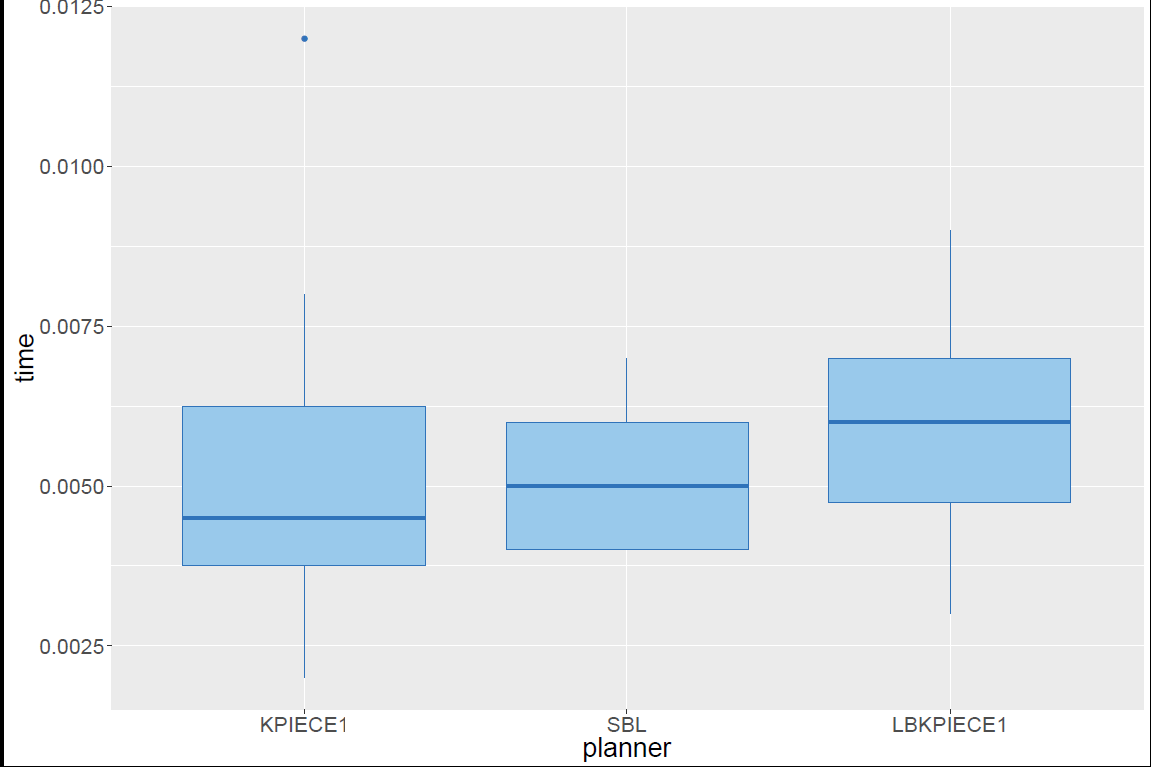
\includegraphics[width=0.8\textwidth,scale=0.6]{images/plan3uop.png}}
	\caption{Time of Planning SBL,KPIECE1,LBKPIECE1: Unoptimized}
	\label{fig:tc5}
\end{figure}
\begin{figure}[!htbp] %  figure placement: here, top, bottom, or page
	\centering
	\frame{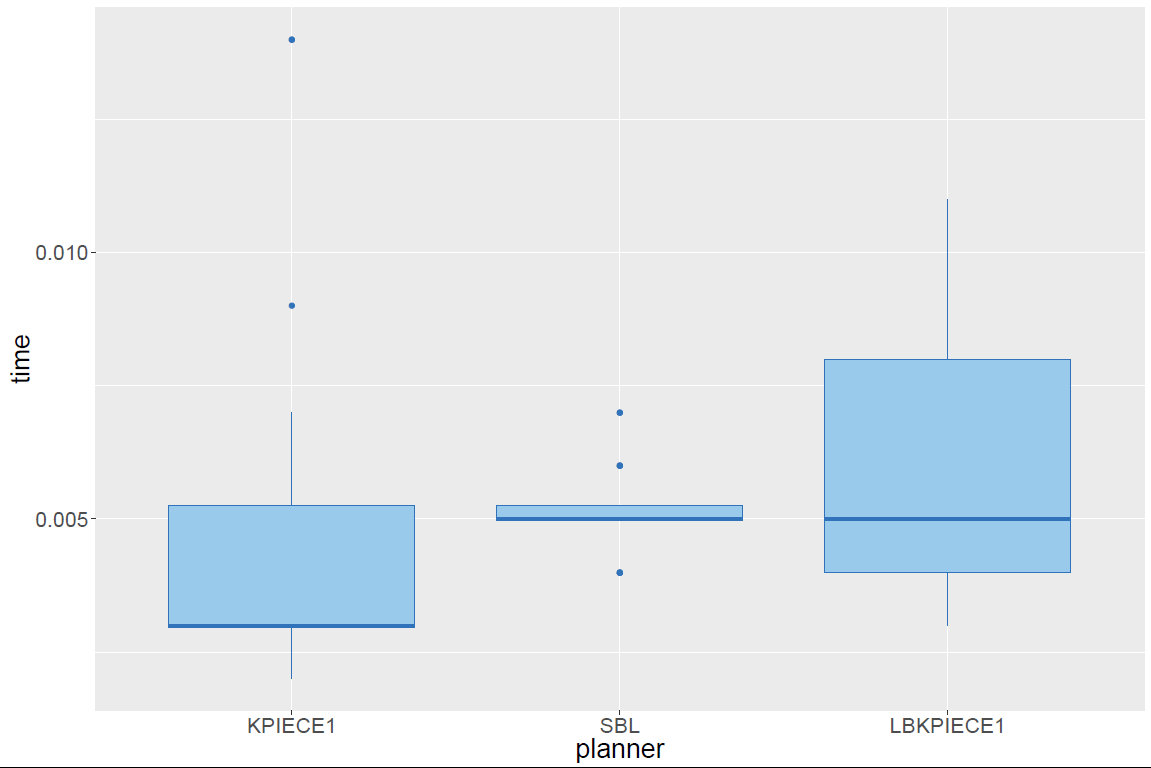
\includegraphics[width=0.8\textwidth,scale=0.6]{images/plan3op.png}}
	\caption{Time of Planning SBL,KPIECE1,LBKPIECE1: Optimized}
	\label{fig:tc6}
\end{figure}
From the plot pairs presented (\ref{fig:tc1} and \ref{fig:tc2}), (\ref{fig:tc3} and \ref{fig:tc4}) and (\ref{fig:tc5} and \ref{fig:tc6}), we can conclude that the planning time remains largely unaffected, by the optimization. For RRT* it was already explained, that because it tries to optimize continuously, it runs for the entire length of planning duration. 

\begin{figure}[!htbp] %  figure placement: here, top, bottom, or page
	\centering
	\frame{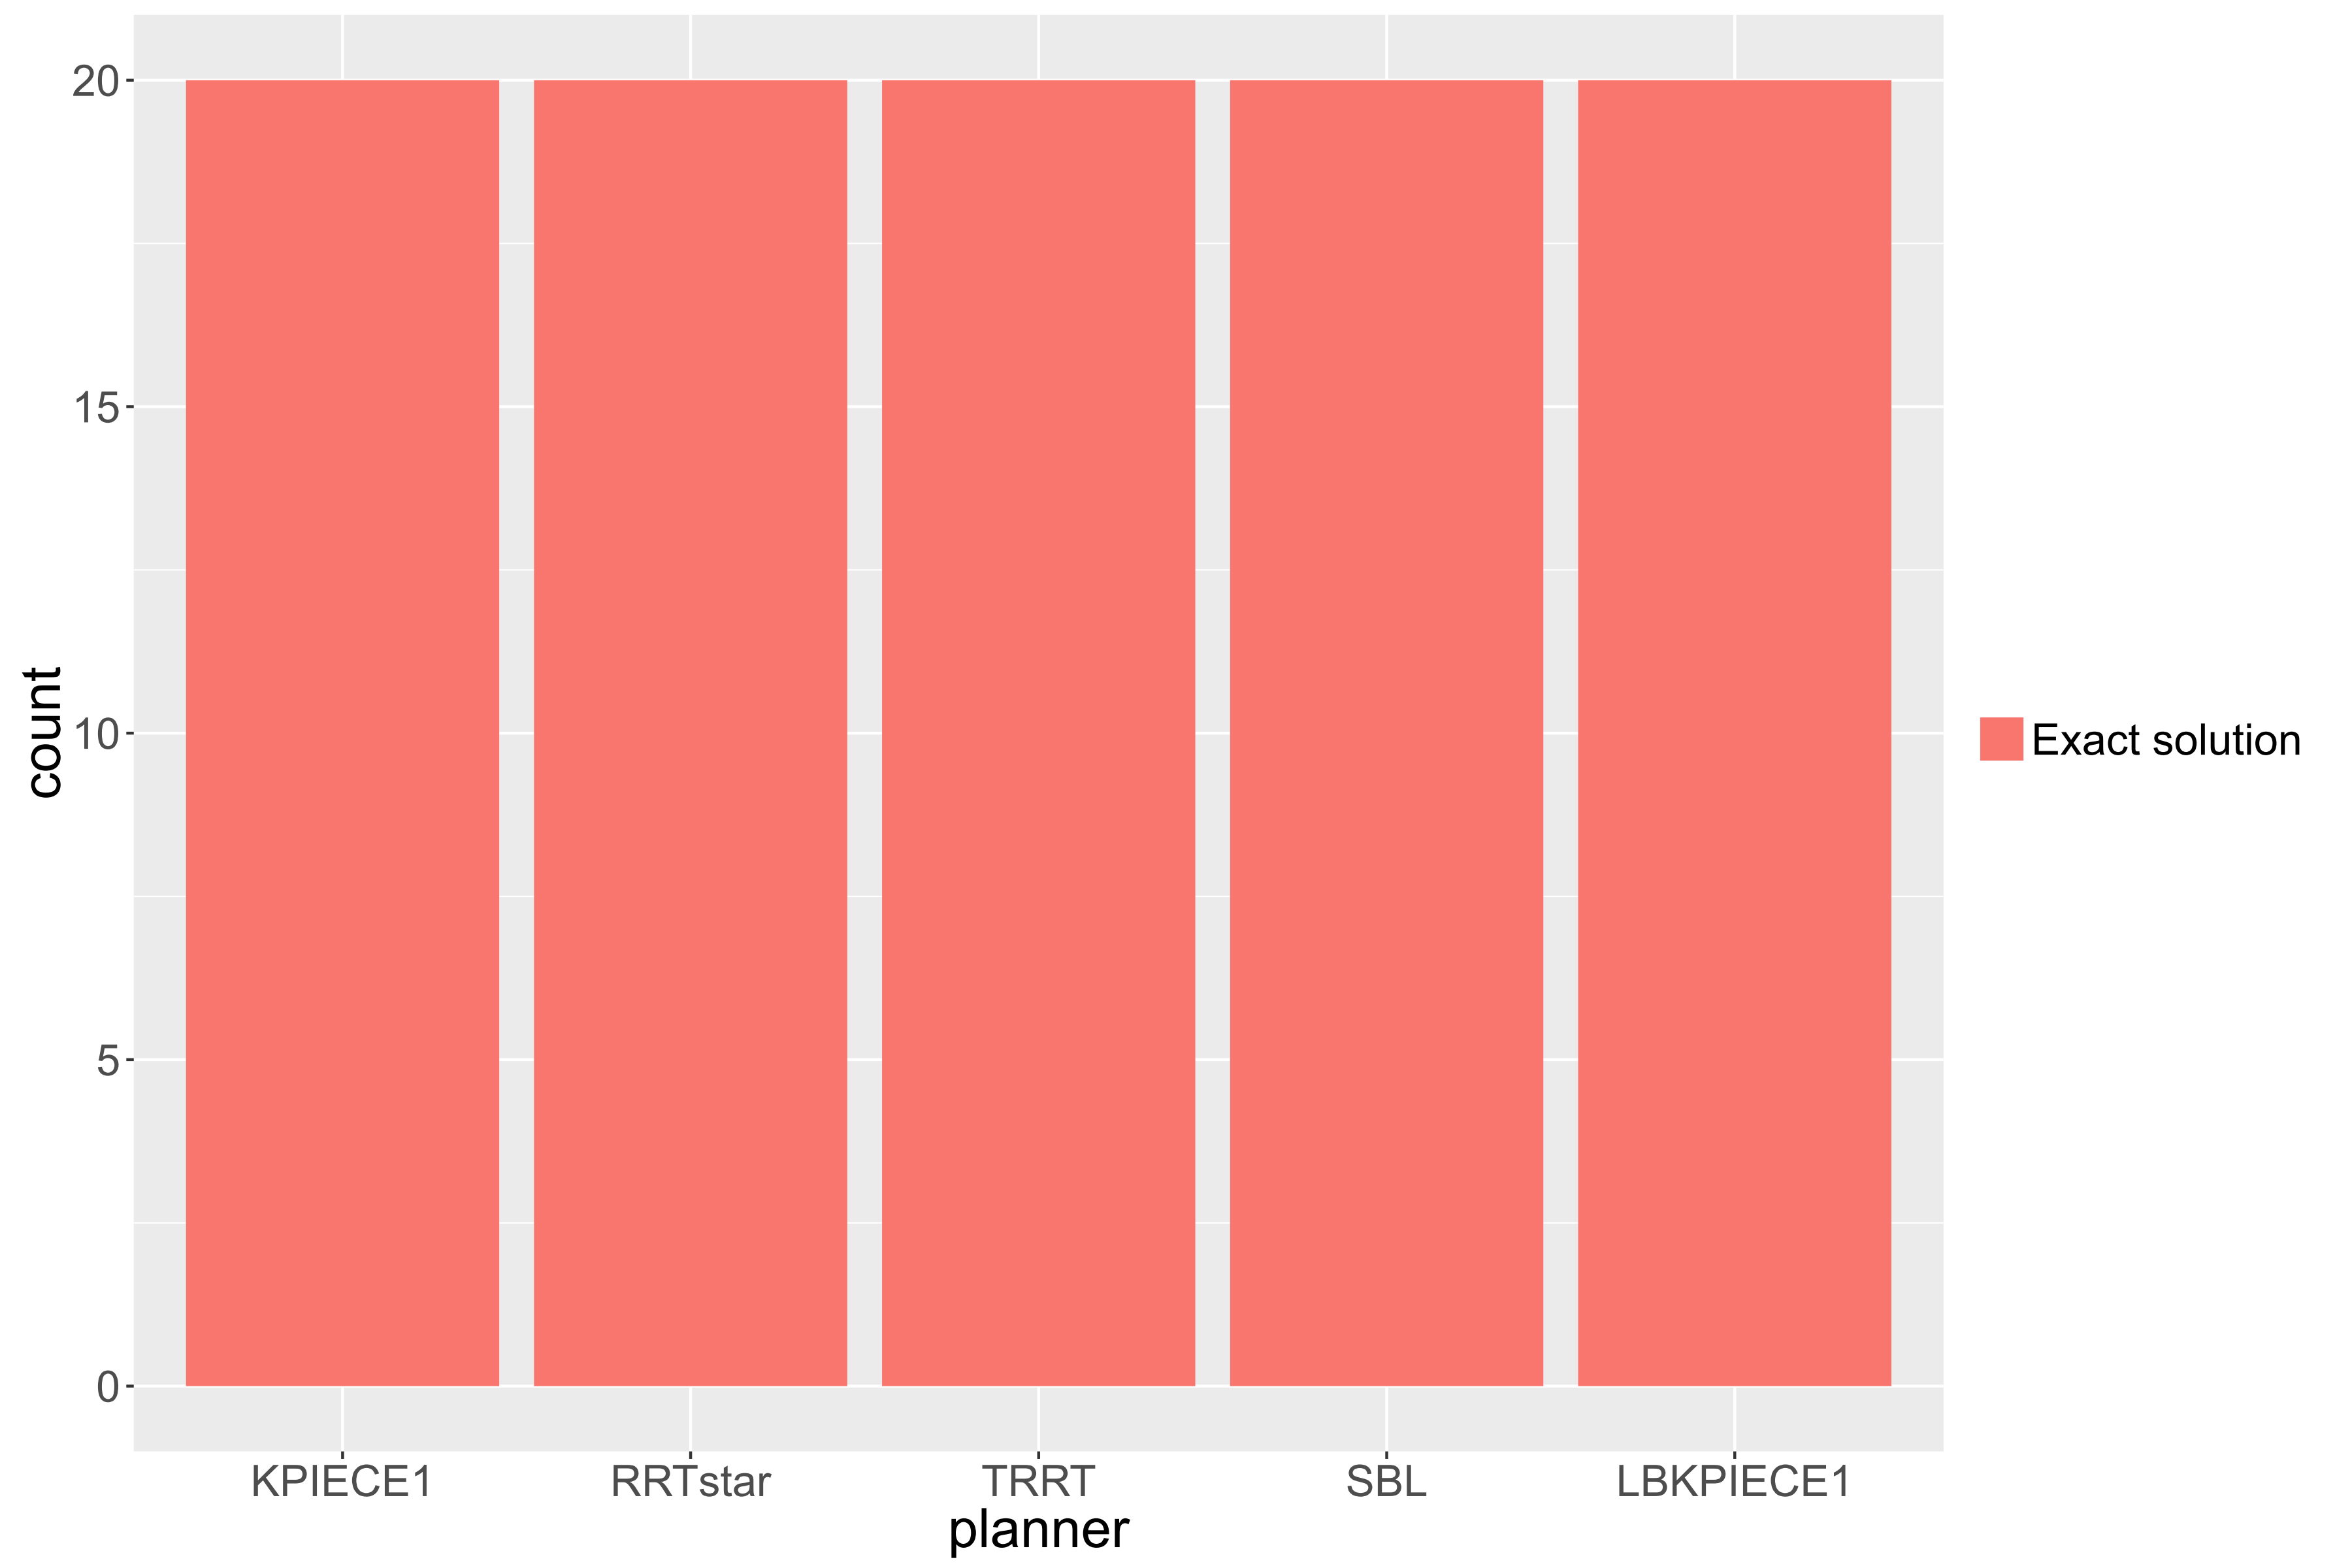
\includegraphics[width=0.8\textwidth,scale=0.6]{images/status_uopt.png}}
	\caption{Status of Planning: Unoptimized}
	\label{fig:stc1}
\end{figure}
\begin{figure}[!htbp] %  figure placement: here, top, bottom, or page
	\centering
	\frame{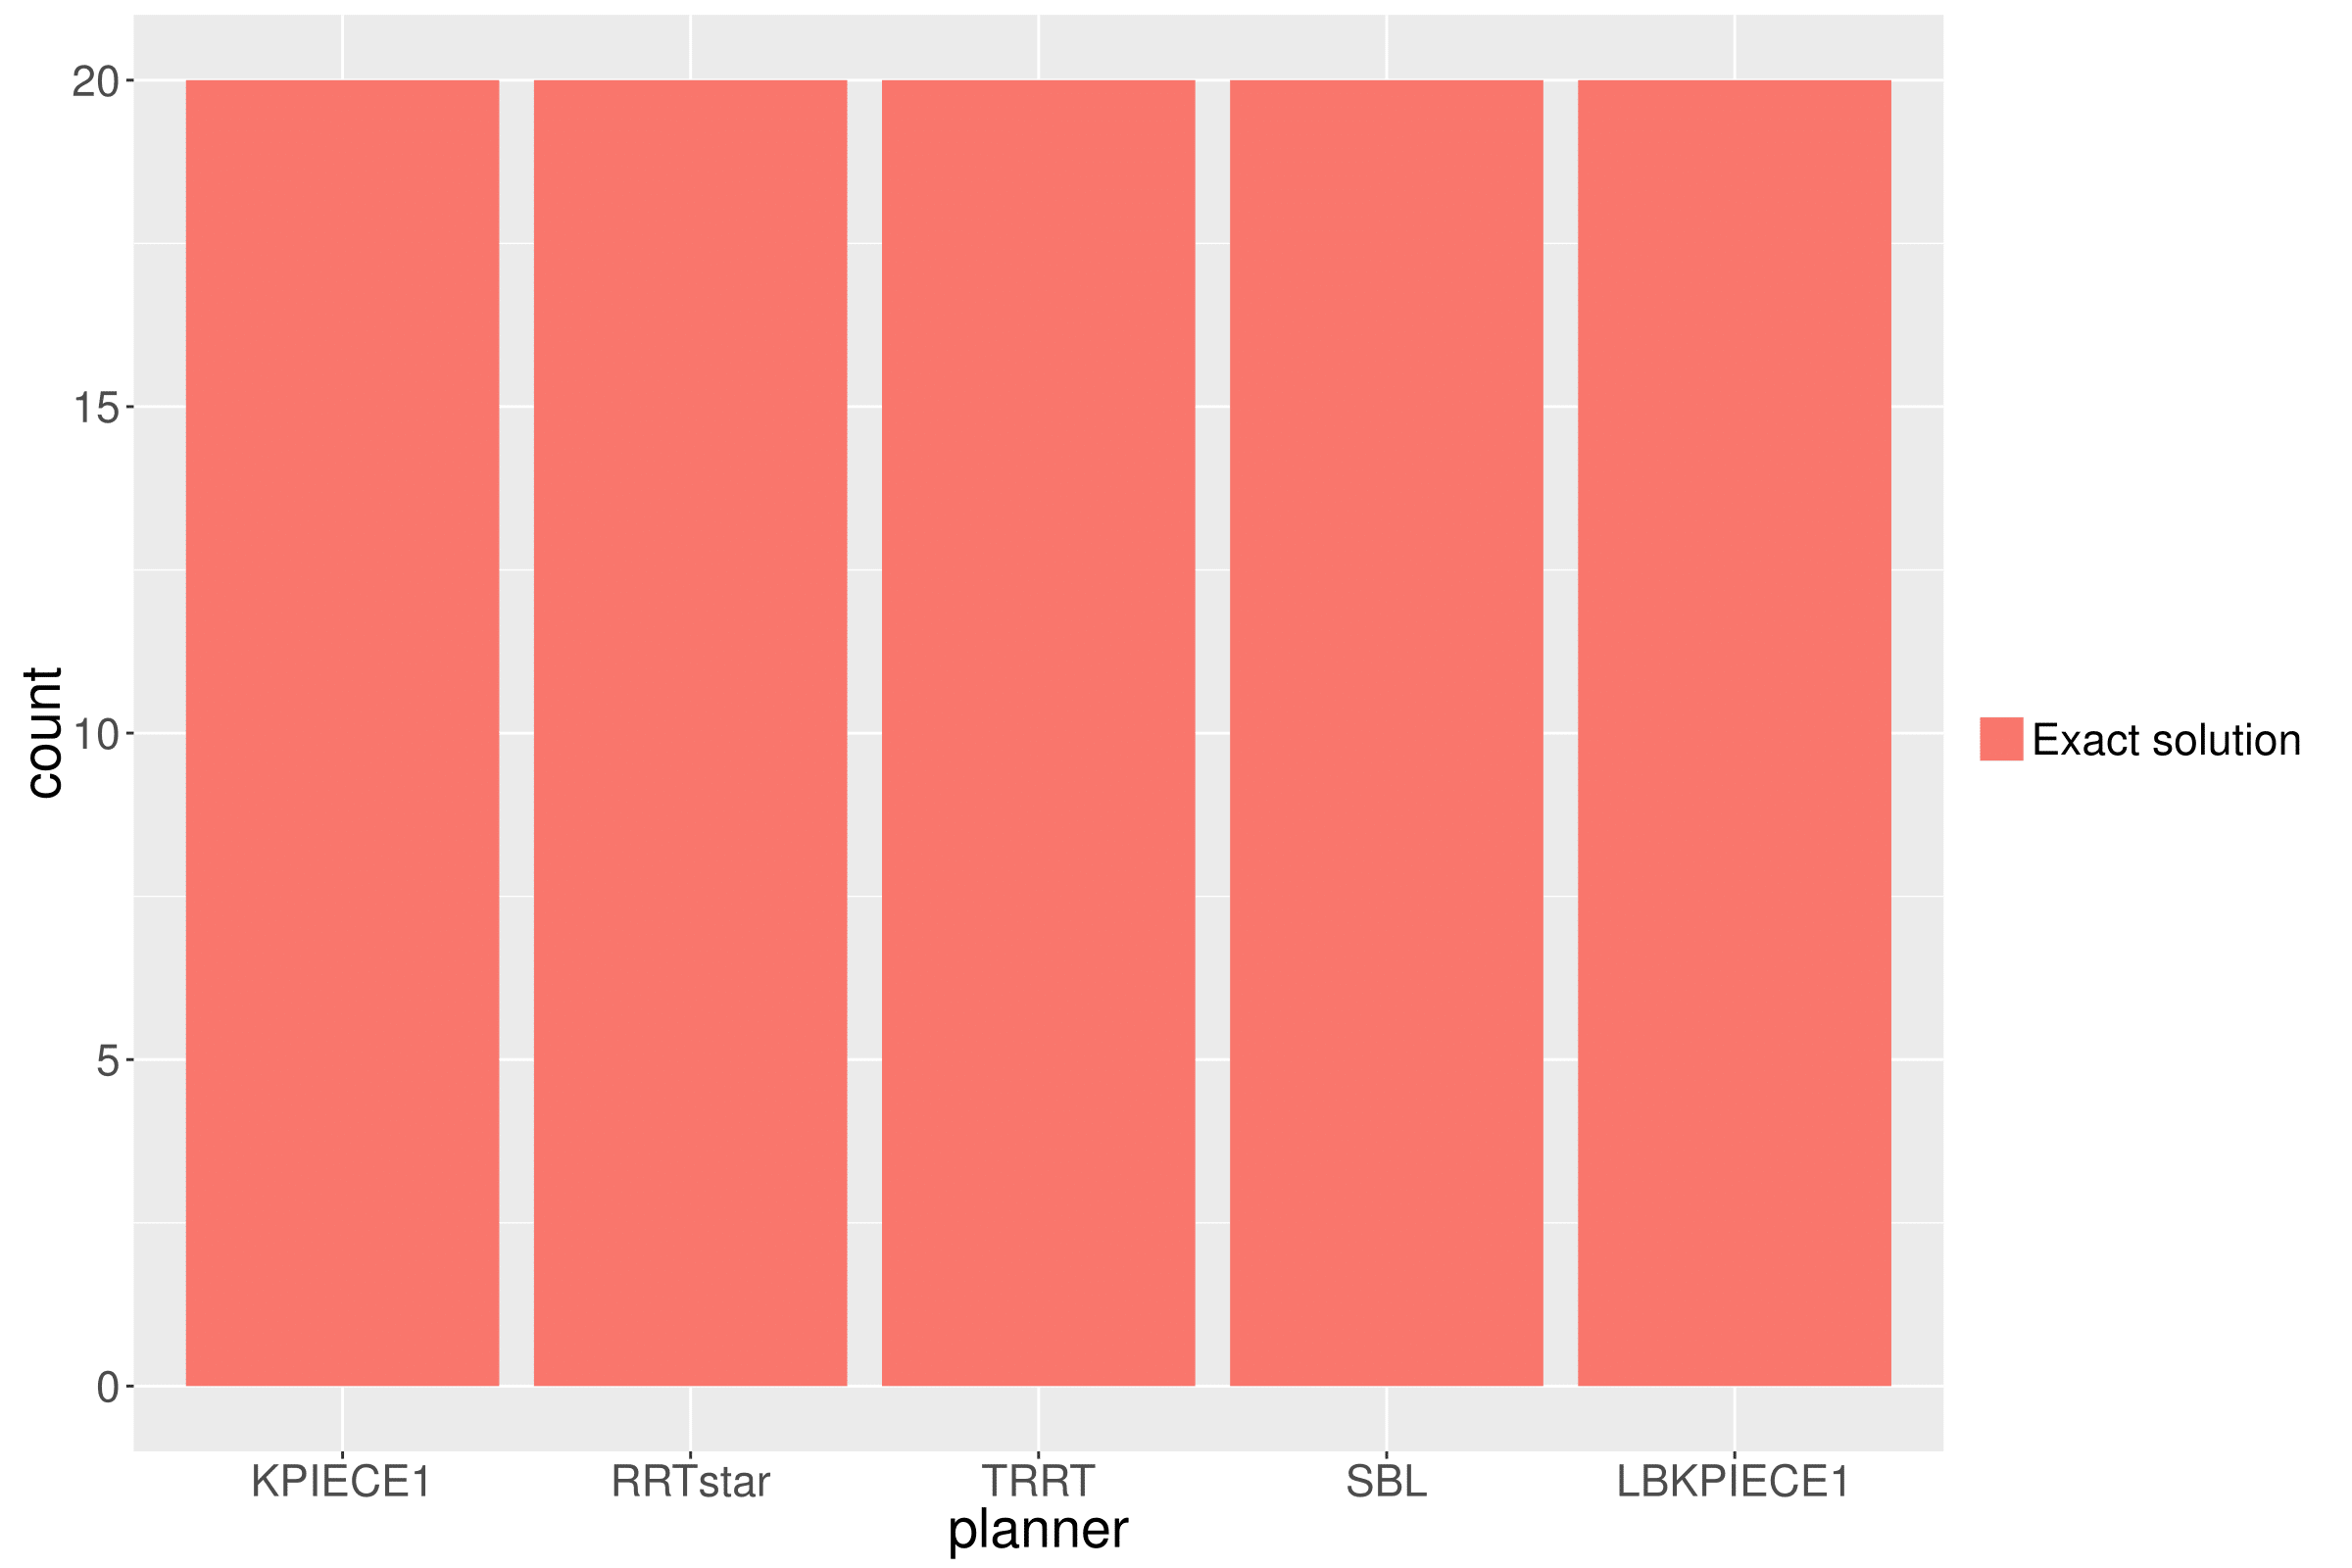
\includegraphics[width=0.8\textwidth,scale=0.6]{images/status_opt.png}}
	\caption{Status of Planning: Optimized}
	\label{fig:stc2}
\end{figure}
From figures (\ref{fig:stc1} and \ref{fig:stc2}), we can conclude that for both use cases, the planners were able to solve with 100\% accuracy.

A key measure of a planner's performance is the, how much cost optimization it can perform, \citet{sucan2012the-open-motion-planning-library}. Since the benchmarking library currently records the best cost found only for the RRT*, so the data for RRT* is presented in figure 

\begin{figure}[!htbp] %  figure placement: here, top, bottom, or page
	\centering
		\frame{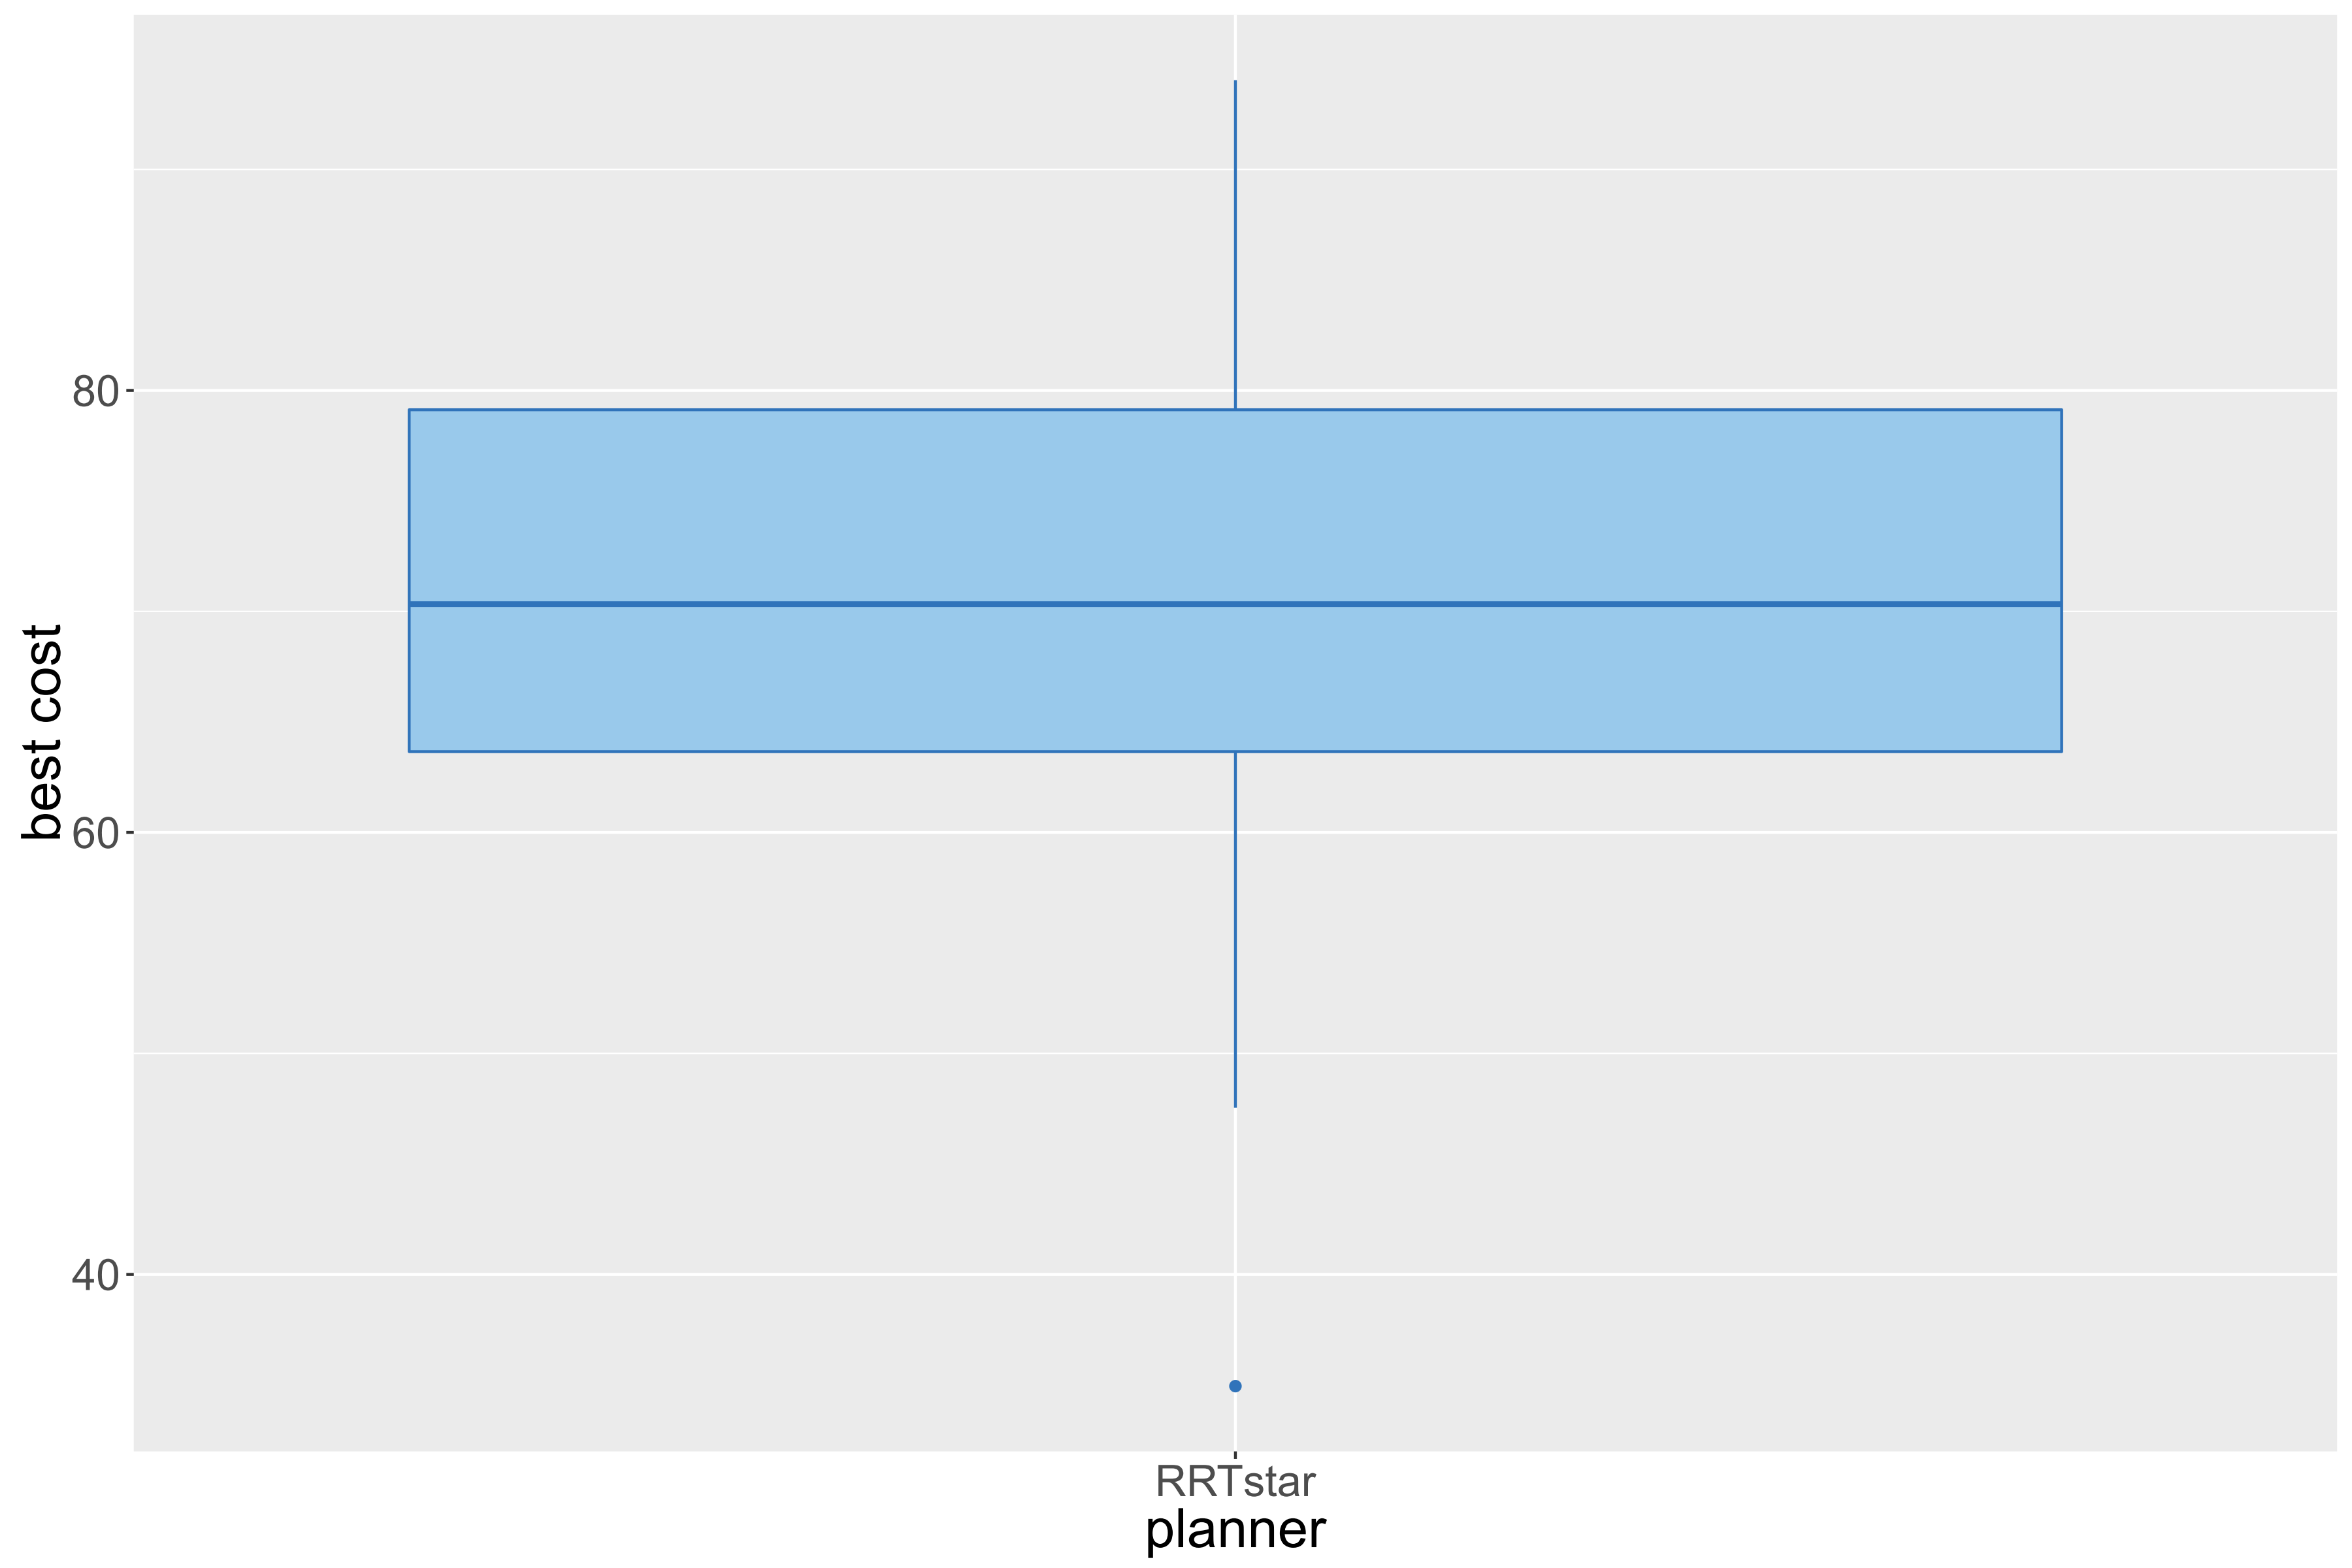
\includegraphics[width=0.8\textwidth,scale=0.6]{images/bestcost_uopt.png}}
		\caption{Best Cost of Planning Instance: Unoptimized}
		\label{fig:bc1}
\end{figure}

\begin{figure}[!htbp]
	\centering
		\frame{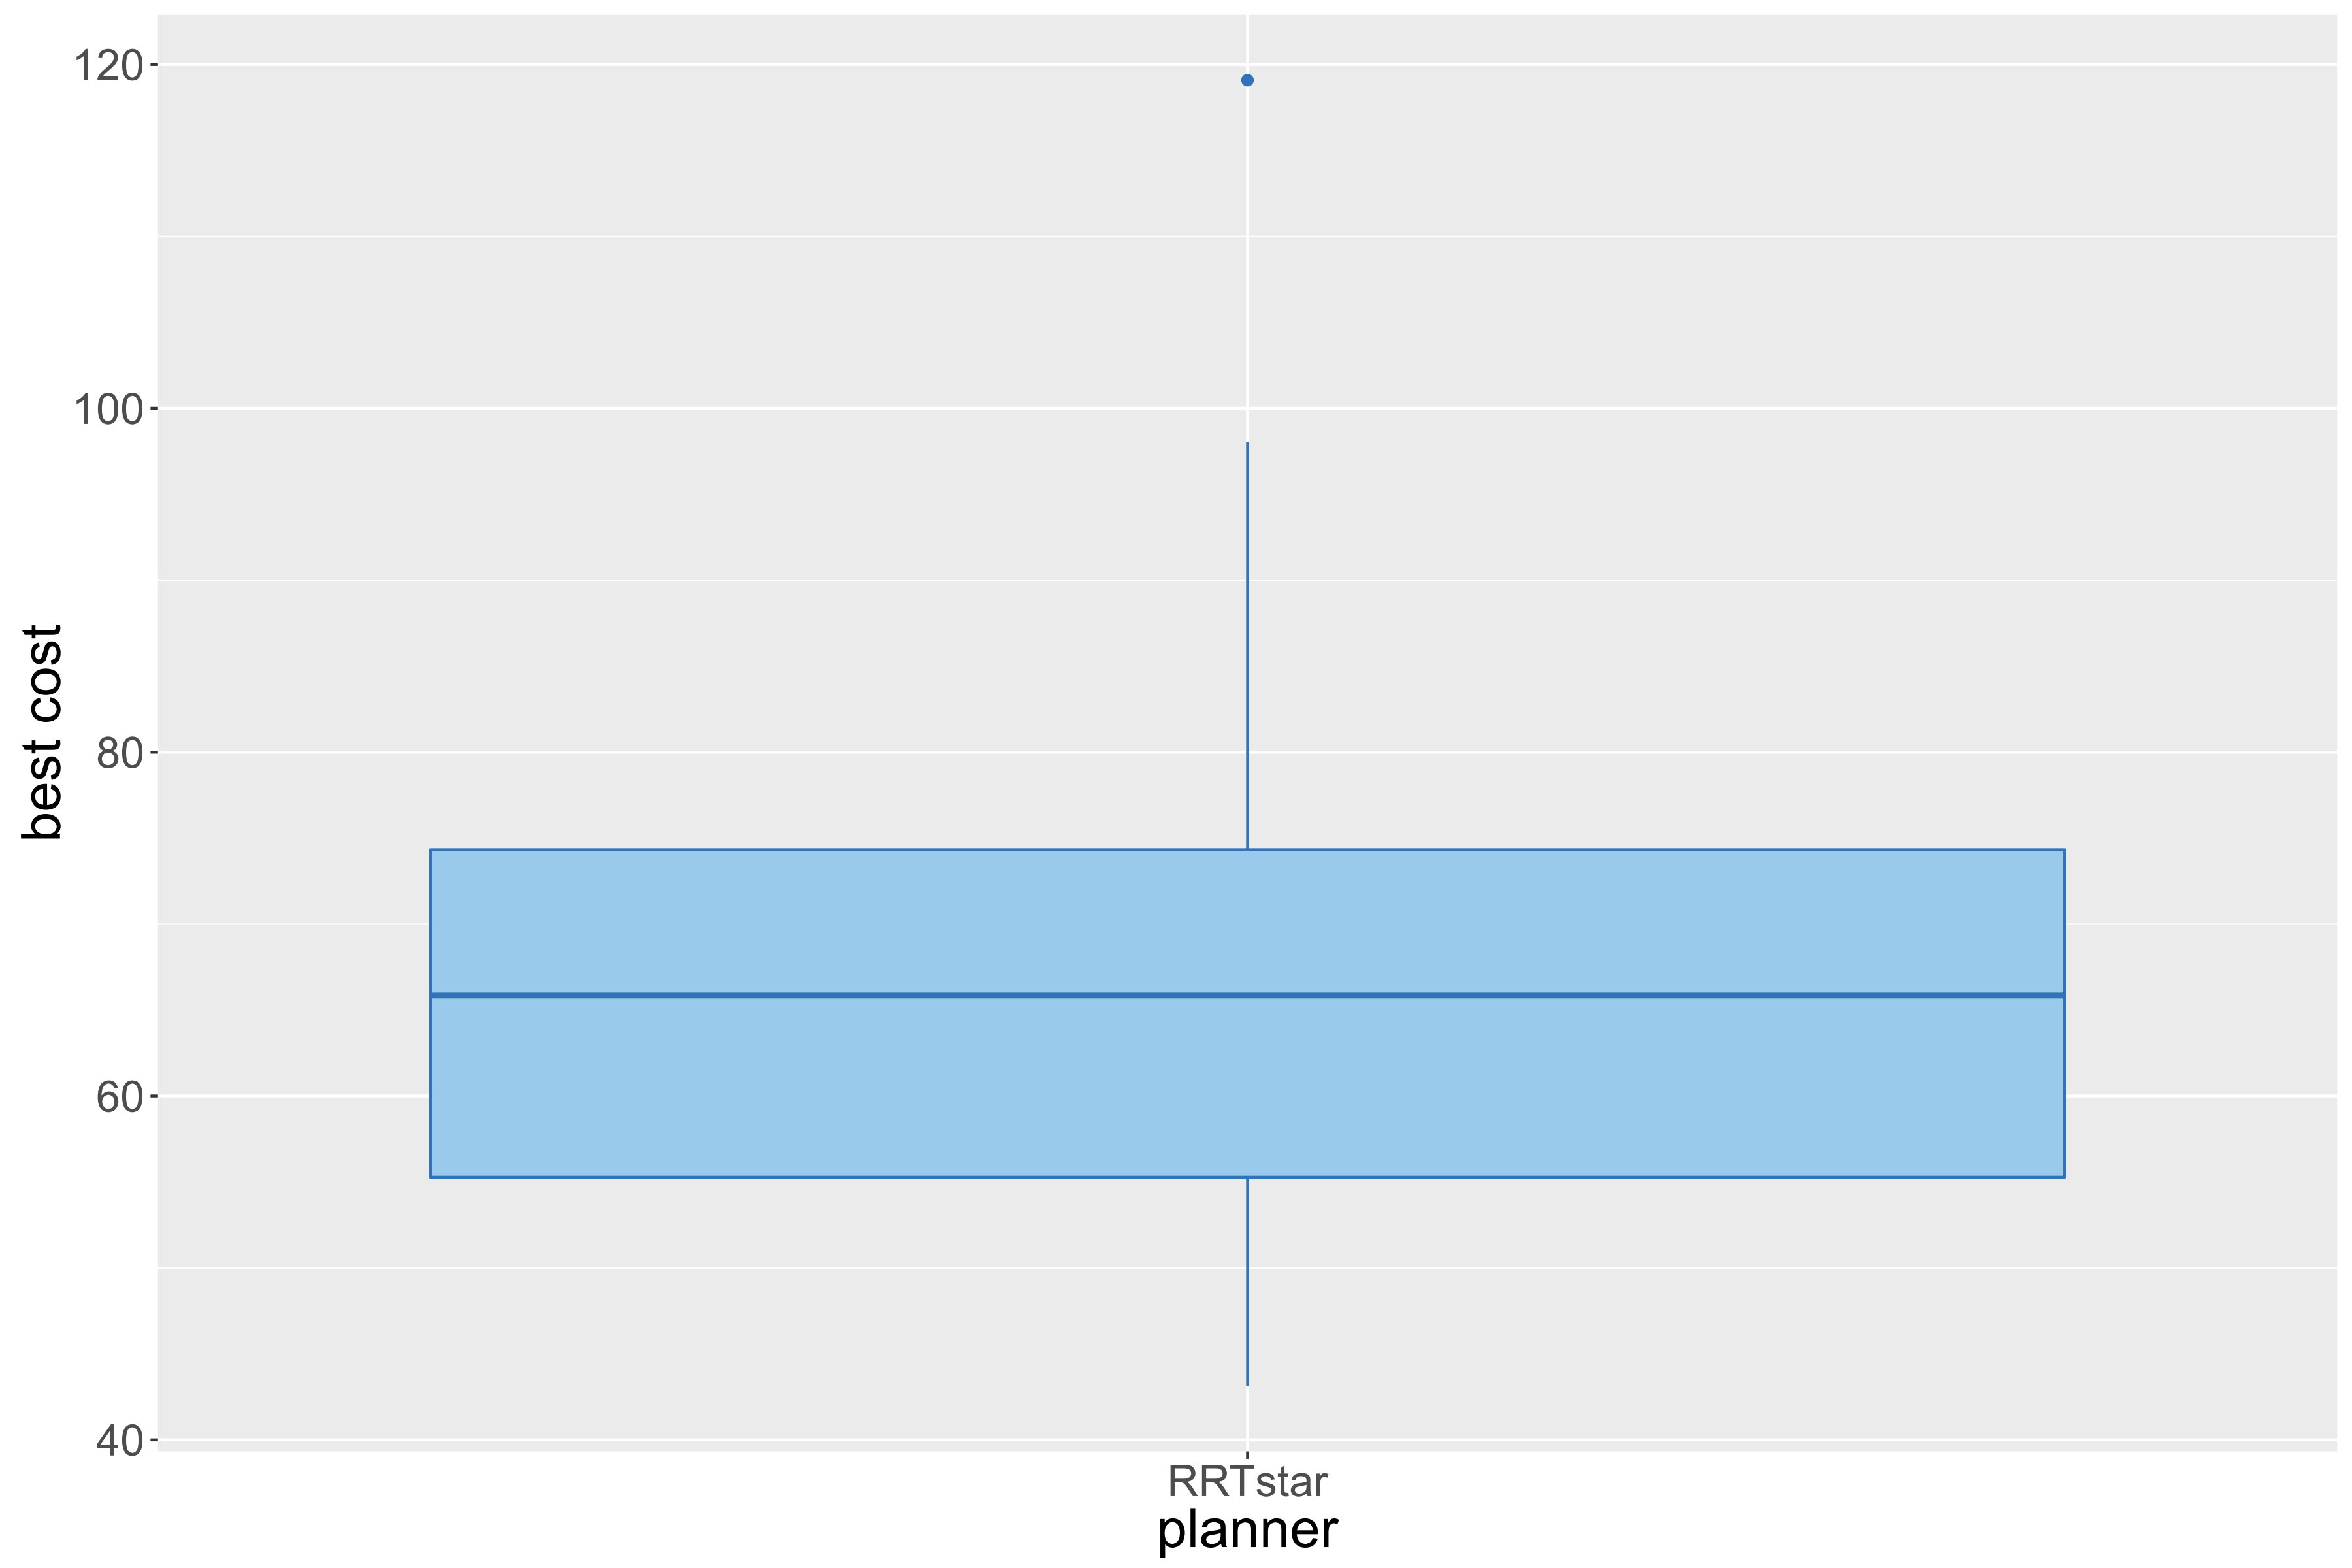
\includegraphics[width=0.8\textwidth,scale=0.6]{images/bestcost_opt.png}}
		\caption{Best Cost of Planning Instance: Using Table Optimization}
	\label{fig:bc2}
\end{figure}

From \ref{fig:bc} we can observe that when we plan with table optimization (plot \ref{fig:bc2}), the median value of the best cost is approximately 65 whereas  when planned without table optimization (plot \ref{fig:bc1}) it is approximately 71. Even the overall range of values generated for optimized use case is lower than the range of values generated for unoptimized use case.

